\documentclass[a4paper,12pt]{article}
\usepackage[T2A]{fontenc}
\usepackage[utf8x]{inputenc}
\usepackage[english,russian]{babel}
\usepackage{amssymb,amsfonts,amsmath,mathtext}
\usepackage[unicode]{hyperref}
\usepackage{listings}
\usepackage{graphicx}
\usepackage{float}
\graphicspath{{images/}}
\newcommand{\anonsection}[1]{\section*{#1}\addcontentsline{toc}{section}{#1}}

\begin{document}

% Титульный лист

\begin{titlepage}
\newpage

\begin{center}

\textit{Министерство науки и высшего образования Российской Федерации \\ 
Федеральное государственное бюджетное образовательное \\
учреждение высшего образования \\
«Московский государственный технический университет \\
имени Н.Э. Баумана (национальный исследовательский университет)» \\
(МГТУ им. Н.Э. Баумана) \\}
\hrulefill
\end{center}

\vspace{2em}

\begin{flushleft}
ФАКУЛЬТЕТ <<Информатика и системы управления>> \\
\vspace{0.5em}
КАФЕДРА <<Программное обеспечение ЭВМ и информационные технологии>>
\end{flushleft}


\vspace{8em}

\begin{center}
\LARGE Лабораторная работа №8 \\
\end{center}

\vspace{1.5em}

\begin{center}
\textsc{Поиск в словаре}
\end{center}

\vspace{6em}

\begin{center}
Головнев Н.В.

\vspace{4em}

ИУ7-54Б
\end{center}

\vspace{\fill}

\begin{center}
Москва 2019
\end{center}

\end{titlepage}

\tableofcontents

% Введение

\newpage
\anonsection{ВВЕДЕНИЕ}
Алгоритмы поиска в словаре - алгоритмы, определяющие наличие найденного в тексте слова в некой коллекции данных, которая называется словарем.

\newpage
\anonsection{ПОСТАНОВКА ЗАДАЧИ}
Необходимо реализовать алгоритм поиска слов в словаре. Эффективность алгоритма должна составлять не более $\log_2N$, где N - размер сегмента словаря (кол-во слов), в котором производится поиск.

\newpage
\section{АНАЛИТИЧЕСКАЯ ЧАСТЬ}
\subsection{Описание алгоритма}
Пусть V - заданный алфавит. % Доделай
Словарь можно представить как древовидную структуру вида: \\
% Добавь сюда ещё одну картинку
Так, например, словарь из слов <<aab>>, <<abc>>, <<abda>> можно представить как:
\begin{figure}[H]
\center{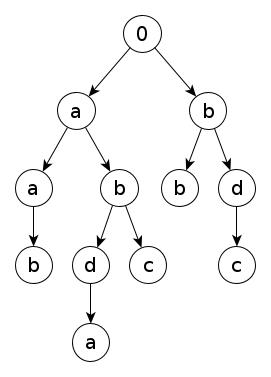
\includegraphics[scale=0.5]{treexample.png}}
\caption{Структура словаря из примера}
\label{images:tree2}
\end{figure}

\newpage
\subsection{Вывод}
Аналитически 

% Конструкторская часть

\newpage
\section{КОНСТРУКТОРСКАЯ ЧАСТЬ}

\subsection{Разработка алгоритма}
На вход у алгоритма передаются в качестве параметров:
\begin{enumerate}
\item Словарь (указатель или ссылка);
\item Строка, которая ищется в словаре;
\item Длина этой строки;
\item Переменная в которую будет записан результат (указатель или ссылка);
\end{enumerate}
Возвращаемое значение: код ошибки (0 в случае успеха, иначе отрицательное значение). \\
Побочные эффекты: изменяется значение переменной результата.

\newpage
\subsection{Схемы алгоритмов}
Ниже представлена схема алгоритма поиска в словаре (словарь представлен как дерево символов).
\begin{figure}[H]
\center{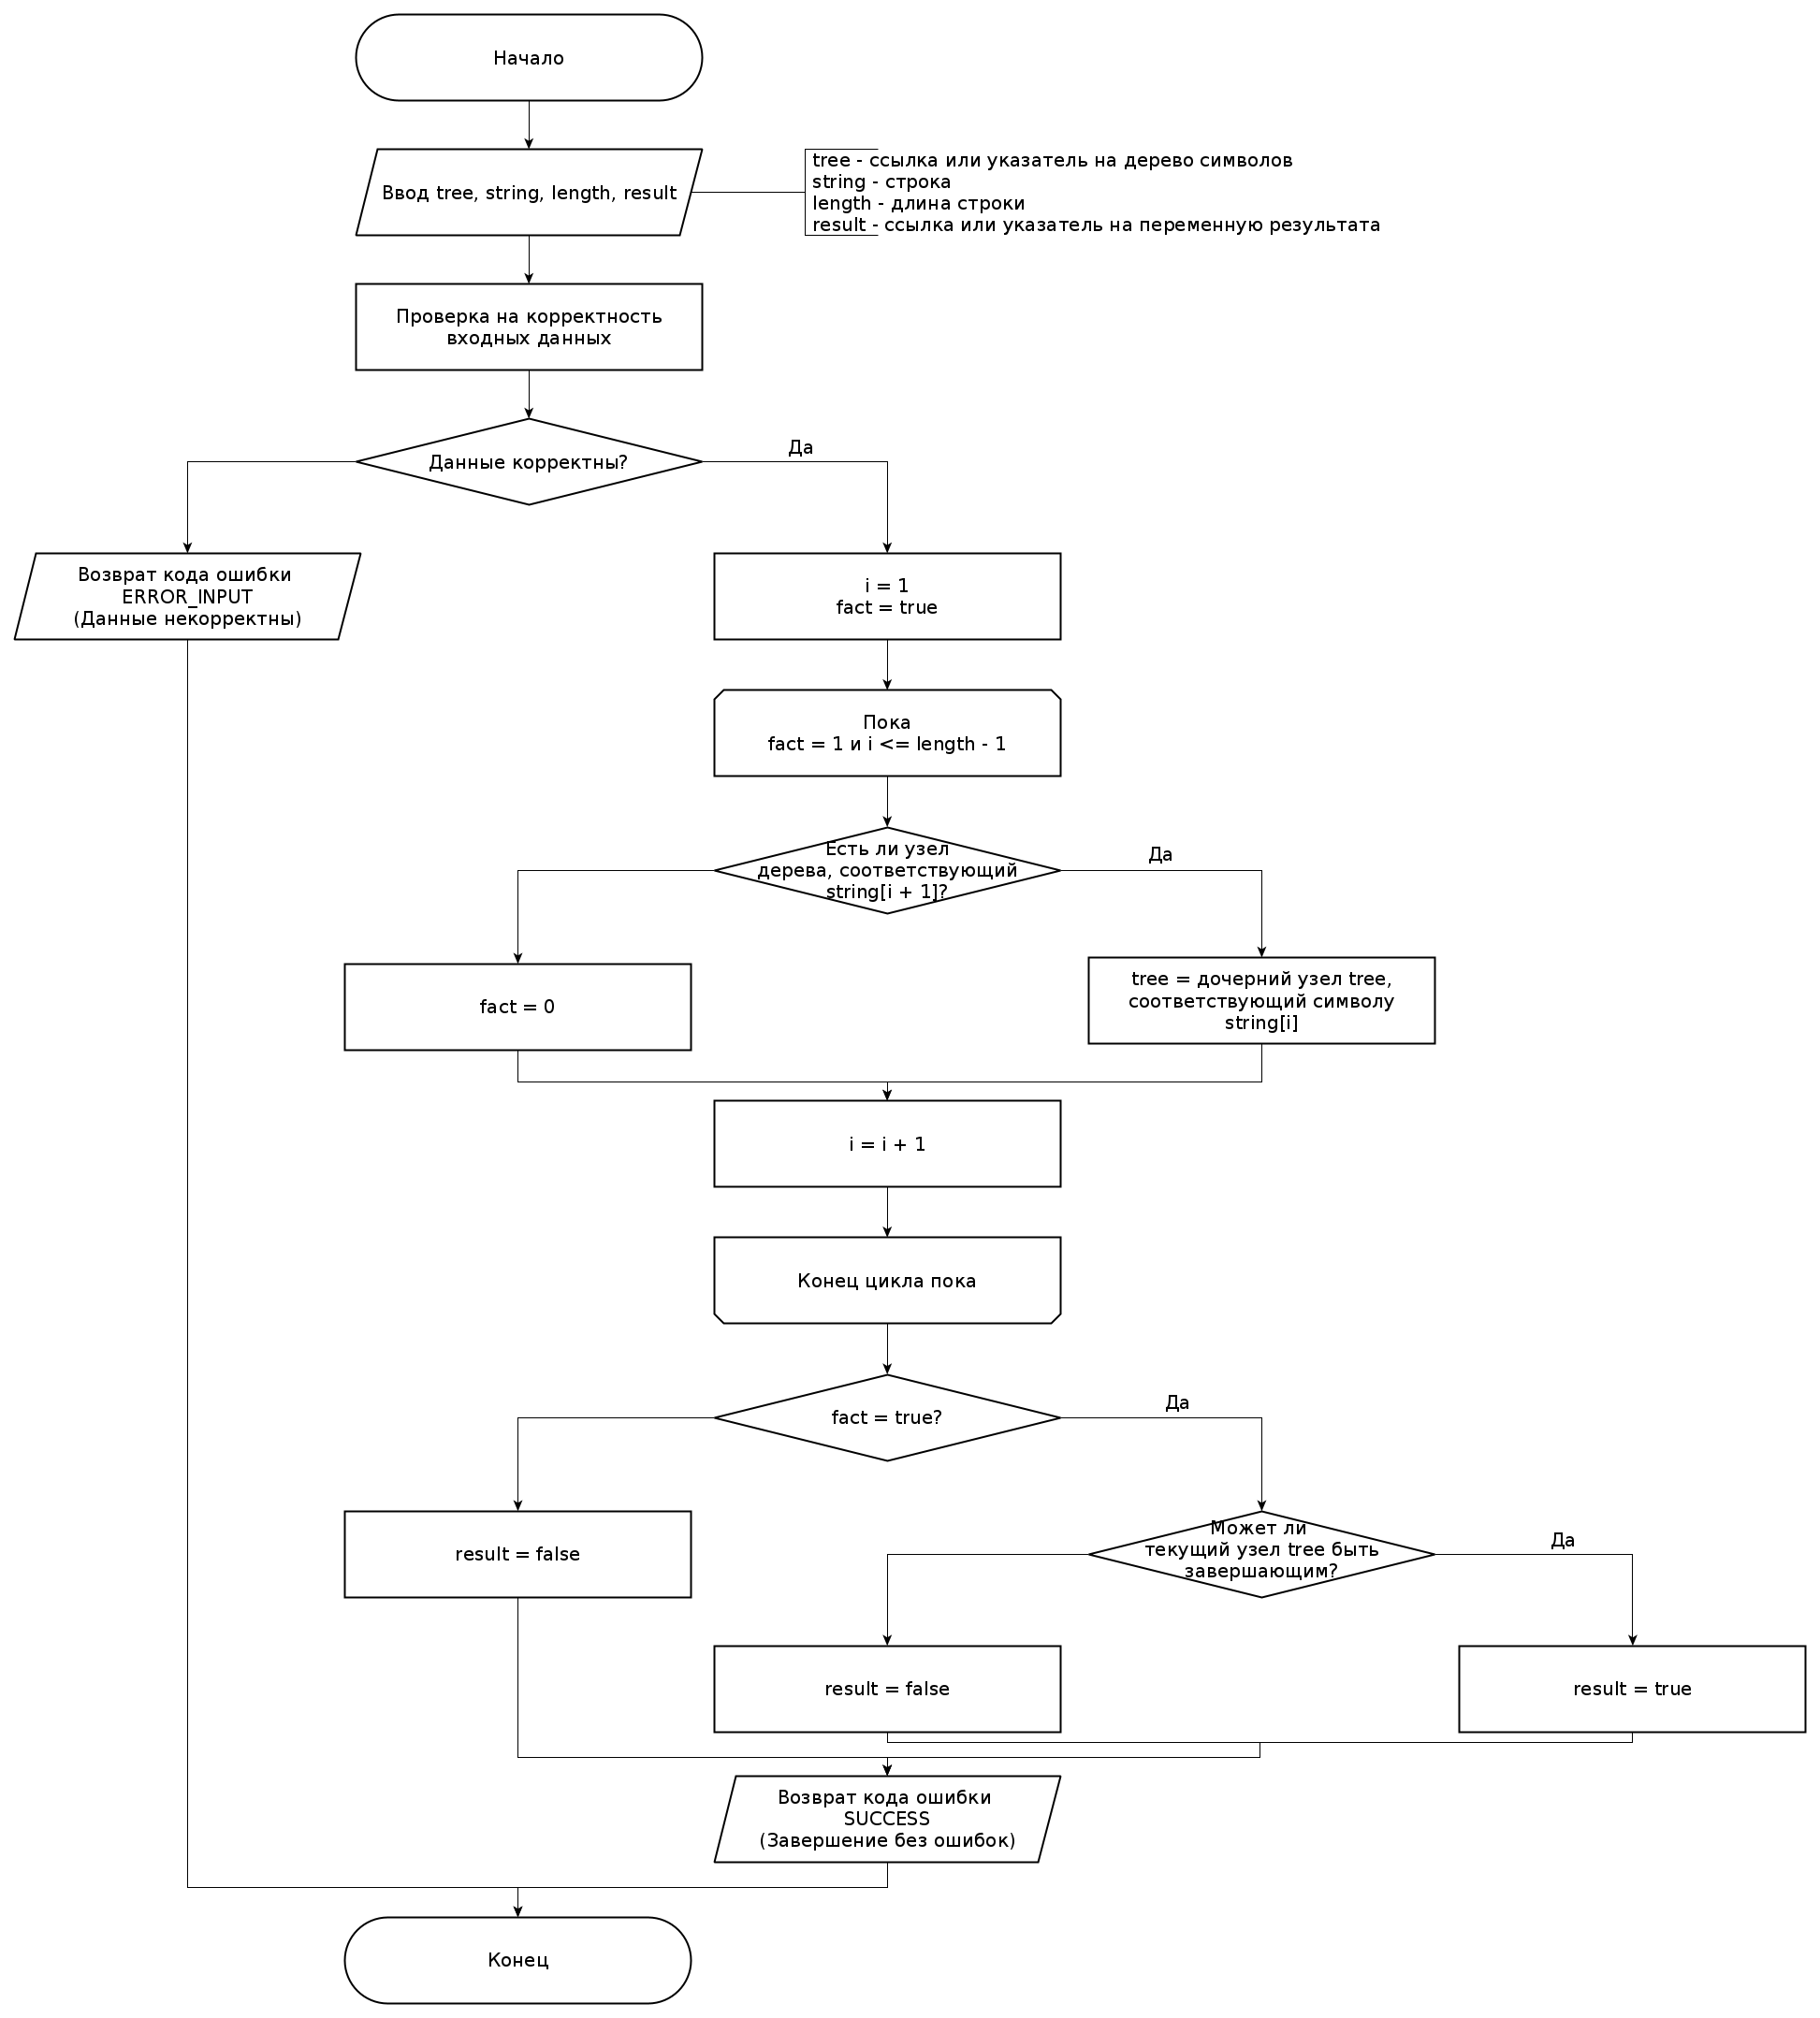
\includegraphics[scale=0.22	]{dictsearching.png}}
\caption{Схема алгоритма поиска в словаре}
\label{images:scheme1}
\end{figure}

\newpage
\subsection{Вывод}
На основе аналитических данных были разработаны требования к разрабатываемым алгоритмам.


\newpage
\section{ТЕХНОЛОГИЧЕСКАЯ ЧАСТЬ}
\subsection{Требования к программному обеспечению}
Программа должна работать на операционной системе Arch Linux. 
Программа должна запускаться из консоли (или терминала) следующей командой:\\
\textit{./app.exe dictionary.txt text.txt} \\
\textit{app.exe} - само приложение. \textit{dictionary.txt} - файл со словами, которые загружаются словарь. На каждой строке должно располагаться одно слово без разделительных знаков. \textit{text.txt} - файл с текстом, в котором ищутся слова, отсутствующие в словаре.
На выход программа должна печатать все слова, не найденные в этом словаре.

\newpage
\subsection{Средства реализации}
Для реализации данных алгоритмов был выбран язык программирования С, компилятор gcc и некоторые функции из библиотеки glibc (memcpy, malloc и тд...). \\

\newpage
\subsection{Листинг кода}
Ниже приведена реализация алгоритма на С.\\
\lstdefinestyle{customc}{
  belowcaptionskip=1\baselineskip,
  breaklines=true,
  frame=L,
  xleftmargin=\parindent,
  language=C,
  showstringspaces=false,
  basicstyle=\footnotesize\ttfamily
}
\lstinputlisting[captionpos=b, caption=\label{listings:listing1}Реализация алгоритма поиска в словаре(\ref{images:scheme1}), style=customc]{listing1.c}
\lstinputlisting[captionpos=b, caption=\label{listings:listing2}Структура узла дерева, style=customc]{listing2.c}
\newpage
\subsection{Вывод}
Используя язык программирования C, в ходе практической работы был спроектирован и написан алгоритм поиска в словаре.

\newpage
\section{ЭКСПЕРИМЕНТАЛЬНАЯ ЧАСТЬ}
\subsection{Характеристики аппаратного и программного обеспечения}
% Часть которую никогда нельзя менять
Тестирование приложения проводилось на машине со следующими характеристиками:\\
\begin{itemize}
\item Процессор Intel® Core™ i7-7700HQ;
\item Оперативная память 16 ГБ;
\item Операционная система - Arch Linux с рабочим окружением Cinnamon.
\end{itemize}

\newpage
\subsection{Примеры работы}
На Рис. \ref{images:example}, предсавленном ниже, демонстрируется работа приложения. Запуск приложения осуществляется из эмулятора терминала в Arch Linux.
\begin{figure}[h]
\center{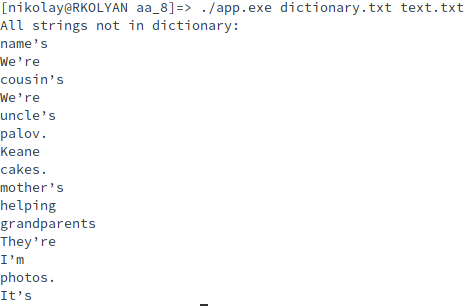
\includegraphics[scale=0.5]{example.png}}
\caption{Пример работы приложения}
\label{images:example}
\end{figure}

\newpage
\subsection{Оценка затрачиваемой памяти}
Размер памяти (в байтах) $M$, выделенной под словарь можно вычислить по формуле:\\
\begin{equation}
M =  \sum_{i = 0}^{\vert V \vert} T_i + P * \vert V \vert
\end{equation}
где:\\
\begin{equation}
T_i = \left\{
\begin{array}{ll}
\vert V \vert * \alpha + \sum_{j = 0}^N T_{ij} + \beta + P\text{,} & \text{if } T_i \text{ exists} \\
0\text{,} & \text{if } T_i \text{ not exists} \\
\end{array}
\right.
\end{equation}
$V$ - заданный алфавит, \\
$\alpha$ - размер символа в байтах, \\
$\beta$ - размер переменной счетчика(если тип integer - 4 байт),\\
$N$ - кол-во дочерних узлов дерева словаря (значение счетчика), \\
$P$ - память, выделяемая под указатели.

\newpage
\subsection{Вывод}
В ходе эксперимантольной части работы было протестирована работа приложения. Была проведенка оценка затрачиваемой памяти этого алгоритма. 

\newpage
\anonsection{ЗАКЛЮЧЕНИЕ}
Поиск в словаре в основном нужен для проверки орфографии в редакторах текста. Также, он ускоряет написание программ в интегрированных средствах разработки путем автоподставления слов (переменных, функций и тд).

\newpage
\anonsection{СПИСОК ИСТОЧНИКОВ}
\begin{itemize}
\item \label{site:wikipedia}https://ru.wikipedia.org/wiki/
\item \label{site:habr}https://habr.com/ru/post/422085/
\end{itemize}

\end{document}
